% Appendix: only what is needed to check the claims of the main text.
% Everything else is in supplement.tex (built to supplement.pdf).

\noindent The appendices contain what is needed to check the claims of the
main text. Further tables and settings are in the
supplementary material that follows them; references of the form S1 or
Table~S1 are to that supplement. The code, the frozen protocol and the logs
of every run are at \repourl.

\section{What was fixed when}
\label{app:fixed-when}

The evidential weight of a result depends on
when it was fixed, and Table~\ref{tab:fixed-when} classifies our results
accordingly. The prediction of single rounds belongs to the first row.
Results in the third row carried a prediction or a threshold that was
recorded in the repository before the corresponding numbers were computed.
The ladder is in the fourth row: its rules were recorded before any of its
code was written, but no outcome was predicted. Results in the last row are
observations made on data we had already seen, experiments designed while
they ran, or rules added after seeing a result. Every run we launched, including those that failed,
is documented in the repository.

\begin{table}[htbp]
\centering
\caption{What was fixed when. Each result is reported in the section given.}
\label{tab:fixed-when}
\small
\begin{tabular}{@{}>{\raggedright\arraybackslash}p{0.3\linewidth}>{\raggedright\arraybackslash}p{0.66\linewidth}@{}}
\toprule
Status & Results \\
\midrule
Fixed before the evaluation runs & The prediction rule and its thresholds; the
  outcome rule; the success criterion (Section~\ref{sec:main-result}) \\
\addlinespace
Planned before the evaluation runs, with no pass mark & The agreement rule
  against the no-carry rule (Section~\ref{sec:confirmed-right}) \\
\addlinespace
Defined after the evaluation runs, and fixed before its own results were
  computed & How often confirmed answers are right
  (Section~\ref{sec:confirmed-right}); the thresholds of the baseline
  (Supplement~\ref{S-app:prediction}) \\
\addlinespace
Rules fixed before any run, with no outcome predicted & The ladder
  (Section~\ref{sec:ladder}): its four arms, the splits, what counts as a
  stage learned, when an arm stops, the threshold of the self-paced arm
  (chosen on the logs of an earlier loop; Appendix~\ref{app:ladder}), the
  three random seeds and their order \\
\addlinespace
Computed afterwards, designed while running, or added after seeing a result
  & Novelty against the size of the change
  (Sections~\ref{sec:novelty-bound} and~\ref{sec:ladder-pace}); the result
  without the basics check (Section~\ref{sec:errors}); the rule for
  repeating a diverged round, written after the first such round on seed~5
  and in place before seeds 6 and~7 (Appendix~\ref{app:ladder});
  the margins of the checks and the variant of the baseline
  (Supplement~\ref{S-app:prediction}) \\
\bottomrule
\end{tabular}
\end{table}


\section{Evidence for Section~\ref{sec:do-the-checks-predict}}
\label{app:evidence}

Figure~\ref{fig:novelty-gain} plots the change in accuracy against novelty
for every evaluation case (Section~\ref{sec:novelty-bound}), and
Table~\ref{tab:teacher-accuracy} gives the accuracy of the teachers' kept
answers (Section~\ref{sec:confirmed-right}).

\begin{figure}[htbp]
\centering
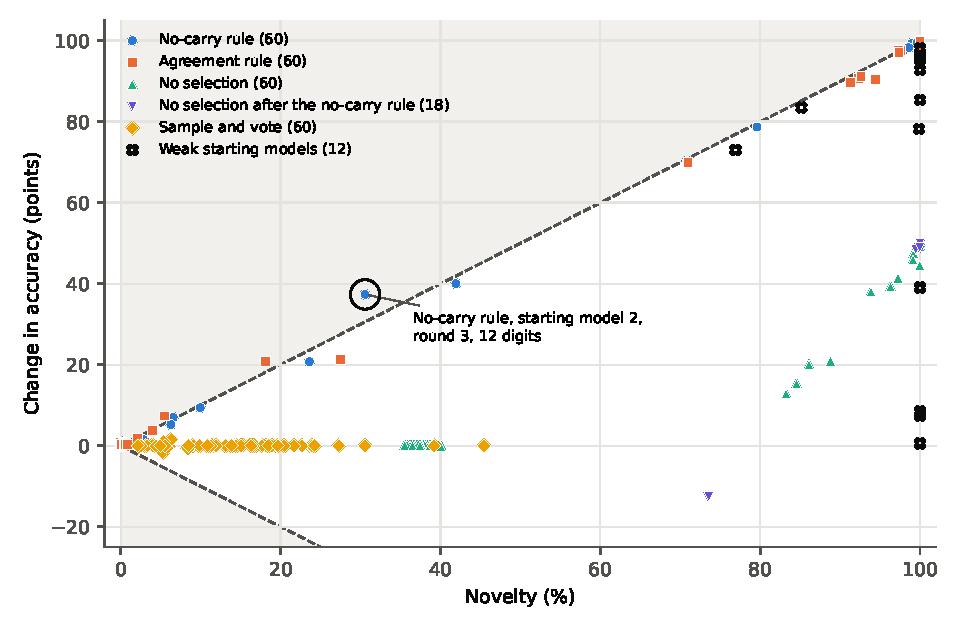
\includegraphics[width=\linewidth]{generated/figure_novelty_gain.pdf}
\caption{Change in accuracy against novelty, one point per evaluation case
  (all \gpNovGainCases, with or without an outcome). Novelty is measured on
  the teacher's kept answers before the round; the change is the accuracy on
  the test problems of that length after the round minus before. Dashed
  lines mark a change equal to plus or minus the novelty, the bound of
  Proposition~\ref{prop:novelty}; points in the shaded area lie outside it.
  The circled case is the only one more than 3 points outside.}
\label{fig:novelty-gain}
\end{figure}

% Built from the macros of generated/numbers.tex (same cells as
% generated/table_teacher_accuracy.tex, without the Cases column).
\begin{table}[htbp]
\centering
\caption{Accuracy of the teachers' kept answers in the evaluation runs,
  measured against the correct sums after all experiments. Each cell is the
  range over cases, in \% of a case's kept answers. The first four rows are
  the \gpTaFullCases{} cases from fully trained starting models. ``Wrong
  but confirmed'' is $\varepsilon$ of Proposition~\ref{prop:agreement}.}
\label{tab:teacher-accuracy}
\small
\begin{tabular}{@{}lcccc@{}}
\toprule
 & Teacher & Confirmed & Wrong but & Accuracy among \\
Teacher & accuracy & share & confirmed & confirmed \\
\midrule
No-carry rule & \gpTaNoCarryAccLow--\gpTaNoCarryAccHigh &
  \gpTaNoCarryConfirmedLow--\gpTaNoCarryConfirmedHigh
  & \gpTaNoCarryWrongConfirmedLow--\gpTaNoCarryWrongConfirmedHigh &
  \gpTaNoCarryAccConfirmedLow--\gpTaNoCarryAccConfirmedHigh \\
Agreement rule & \gpTaAgreementAccLow--\gpTaAgreementAccHigh &
  \gpTaAgreementConfirmedLow
  & \gpTaAgreementWrongConfirmedLow--\gpTaAgreementWrongConfirmedHigh &
  \gpTaAgreementAccConfirmedLow--\gpTaAgreementAccConfirmedHigh \\
No selection & \gpTaNoSelectAccLow--\gpTaNoSelectAccHigh &
  \gpTaNoSelectConfirmedLow--\gpTaNoSelectConfirmedHigh
  & \gpTaNoSelectWrongConfirmedLow--\gpTaNoSelectWrongConfirmedHigh &
  \gpTaNoSelectAccConfirmedLow--\gpTaNoSelectAccConfirmedHigh \\
No selection after the no-carry rule
  & \gpTaNoSelectAfterAccLow--\gpTaNoSelectAfterAccHigh &
  \gpTaNoSelectAfterConfirmedLow--\gpTaNoSelectAfterConfirmedHigh
  & \gpTaNoSelectAfterWrongConfirmedLow--\gpTaNoSelectAfterWrongConfirmedHigh &
  \gpTaNoSelectAfterAccConfirmedLow--\gpTaNoSelectAfterAccConfirmedHigh \\
\midrule
Weak starting models & \gpTaWeakAccLow--\gpTaWeakAccHigh &
  \gpTaWeakConfirmedLow--\gpTaWeakConfirmedHigh
  & \gpTaWeakWrongConfirmedLow--\gpTaWeakWrongConfirmedHigh &
  \gpTaWeakAccConfirmedLow--\gpTaWeakAccConfirmedHigh \\
\bottomrule
\end{tabular}
\end{table}

\section{Details of the ladder}
\label{app:ladder}

\noindent The code and the logs call a split a \emph{cut}.

\paragraph{Splits.} A sum of $n$ digits is split so that the left piece has
$h-1$, $h$ and $h+1$ digits, where $h$ is $n/2$ rounded down. Every piece has
at least 3 digits and is shorter than both lengths its round adds. Up to 12
digits all pieces have at most 7 digits; from 13 digits some split has a
piece of 8 digits or more; from 18 digits every piece of every split has. The
longest piece has 21 digits (Supplement~\ref{S-app:ladder-more},
Table~\ref{S-tab:ladder-splits}). Sums are drawn so that no piece begins with
the digit 0.

\paragraph{One round.} (i) \emph{Measure.} On \gpLadCheckSums{} fresh sums per
new length the model answers directly and through each of the three splits.
From these we log the direct accuracy, the share of sums on which two splits
agree, the confirmed share of the first split's answers, and novelty. Over
all rounds of the third arm the first split's answer was right for
\gpLadCutOneRightLow--\gpLadCutOneRightHigh\% of sums, the confirmed share was
\gpLadConfirmedShareLow--\gpLadConfirmedShareHigh\%, and two splits agreed on
\gpLadAgreedShareLow--\gpLadAgreedShareHigh\%. (ii) \emph{Build.} Fresh sums
are drawn until \gpLadQuota{} answers are kept for each new length, or
\gpLadDrawCapFactor{} times as many sums have been drawn. (iii) \emph{Train}
on the new answers, all answers kept in earlier rounds, and
\gpLadReplayPerLength{} sums at each length from 3 to 7 that the model answers
itself, for \gpLadPasses{} passes over this set and at least \gpLadMinUpdates{}
updates, with the settings of Section~\ref{sec:setup}. (iv) \emph{Test} on
\gpLadTestPerGroup{} held-out sums with a carry across the first split and
\gpLadTestPerGroup{} without, at every length taught so far.

\paragraph{The self-paced arm.} Novelty is the share of the sums on which two
splits agree whose agreed answer differs from the direct answer. A length is
built if novelty is at least \gpLadThreshold\%, or if fewer than
\gpLadMinAgreed{} of the \gpLadCheckSums{} sums have two splits that agree,
since then the teacher, not the student, is the problem. For a length that
is not built, the agreed answers of the measurement are stored and repeated
to the weight of a built length; the number of updates is computed from the
unrepeated examples. The gain of a round at a length is the accuracy on
the test sums after the round minus the direct
accuracy in the measurement before it. Across the three seeds, the highest
novelty at a skipped length was \gpLadSkippedNoveltyHighSeedFive,
\gpLadSkippedNoveltyHighSeedSix{} and \gpLadSkippedNoveltyHighSeedSeven\%.
The \gpLadThreshold\% threshold was chosen before these runs, on the logs of
an earlier loop over 16 to 39 digits. That loop started from a model taught 8
to 15 digits with the no-carry rule and trained on every length whatever its
checks said. It is documented with its logs in the repository, as are further
experiments not reported here.

\begin{table}[htbp]
\centering
\caption{The self-paced arm against the arm that builds answers at every
  length. Shares are the self-paced arm's as a percentage of the other's.
  The difference is in final accuracy, in points, averaged over the lengths
  8 to 39.}
\label{tab:ladder-pace}
\small
\begin{tabular}{@{}lccc@{}}
\toprule
 & Seed 5 & Seed 6 & Seed 7 \\
\midrule
Lengths skipped, of 32 & \gpLadSkippedSeedFive & \gpLadSkippedSeedSix &
  \gpLadSkippedSeedSeven \\
Rounds without training, of 16 & \gpLadRoundsSkippedSeedFive &
  \gpLadRoundsSkippedSeedSix & \gpLadRoundsSkippedSeedSeven \\
Training updates (\%) & \gpLadUpdatesShareSeedFive &
  \gpLadUpdatesShareSeedSix & \gpLadUpdatesShareSeedSeven \\
GPU time (\%) & \gpLadGpuShareSeedFive & \gpLadGpuShareSeedSix &
  \gpLadGpuShareSeedSeven \\
Difference in accuracy (points) & $\gpLadDiffMeanSeedFive$ &
  $\gpLadDiffMeanSeedSix$ & $\gpLadDiffMeanSeedSeven$ \\
Lowest accuracy at a skipped length (\%) & \gpLadSkippedFinalLowSeedFive &
  \gpLadSkippedFinalLowSeedSix & \gpLadSkippedFinalLowSeedSeven \\
\bottomrule
\end{tabular}
\end{table}

\paragraph{Diverged rounds.} A round after which accuracy is below
\gpLadDivergedLevel\% at any length from 3 to 7 digits is trained once
more, from the same weights and on the same examples, with a different batch
order; a second failure ends the arm. This rule was written after the first
such round, in the third arm on seed~5, and that arm was continued under it;
seeds 6 and~7 ran with it from the start. It was triggered
\gpLadDivergedEvents{} times, both in the third arm on seed~5,
and \gpLadDivergedRedosFailed{} of the repeated rounds diverged again. The
arm's first run, which stopped after the first diverged round under the
rules then in force, is reported with the others in the repository.

\begin{figure}[htbp]
\centering
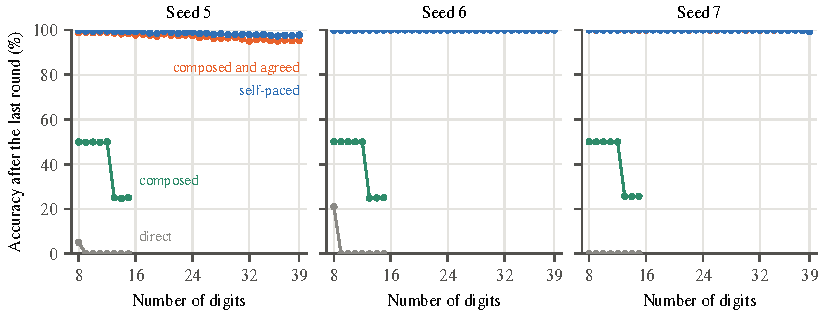
\includegraphics[width=\linewidth]{generated/figure_ladder_accuracy.pdf}
\caption{Accuracy at each length after an arm's last round, for the three
  starting models. The first two arms stopped after stage~1 (8 to 15
  digits).}
\label{fig:ladder}
\end{figure}

\paragraph{Cost.} The three seeds cost \$\gpLadCostSeedFive,
\$\gpLadCostSeedSix{} and \$\gpLadCostSeedSeven{} of GPU time.
